\documentclass{swfulabreport}

\usepackage{zhlipsum}

\swfusetup{%
  Title        ={《单片机原理与接口技术》课程实习}, % 课程名称
  % School =,%
  Subject = {电子信息工程},%
  Grade = 2021,%
  Tutor      ={李俊萩、戴杨}, %指导教师
  Author       ={翟宇轩}, % 作者姓名
  ID           ={20211151007}, % 学号
  Year         ={\the\year},%
  Month        ={\the\month},%
  Date         ={\the\day},%
  Sig  = {\includegraphics[width=12mm]{wangxiaolin}},%
  CommentsDate = {\the\year 年\the\month 月 30 日},%
  Mark      = {100},%
  LabDate   = {\today},%
  LabDays   = {3},%
  % Lab       = {经管楼219},%
}

\begin{document}

\maketitle % 封面

\section{实习的任务、作用和目的}

\zhlipsum[1-3]

\section{实习主要内容(含工具、方法等)}

\zhlipsum[4-6]

\section{程序及仿真}

\subsection{单片机连接扬声器播放单个音符}

单片机 P1.0 引脚接扬声器播放单个音符,从低音哆,一直到超高音嘻。仿真图
如下:

\begin{center}
  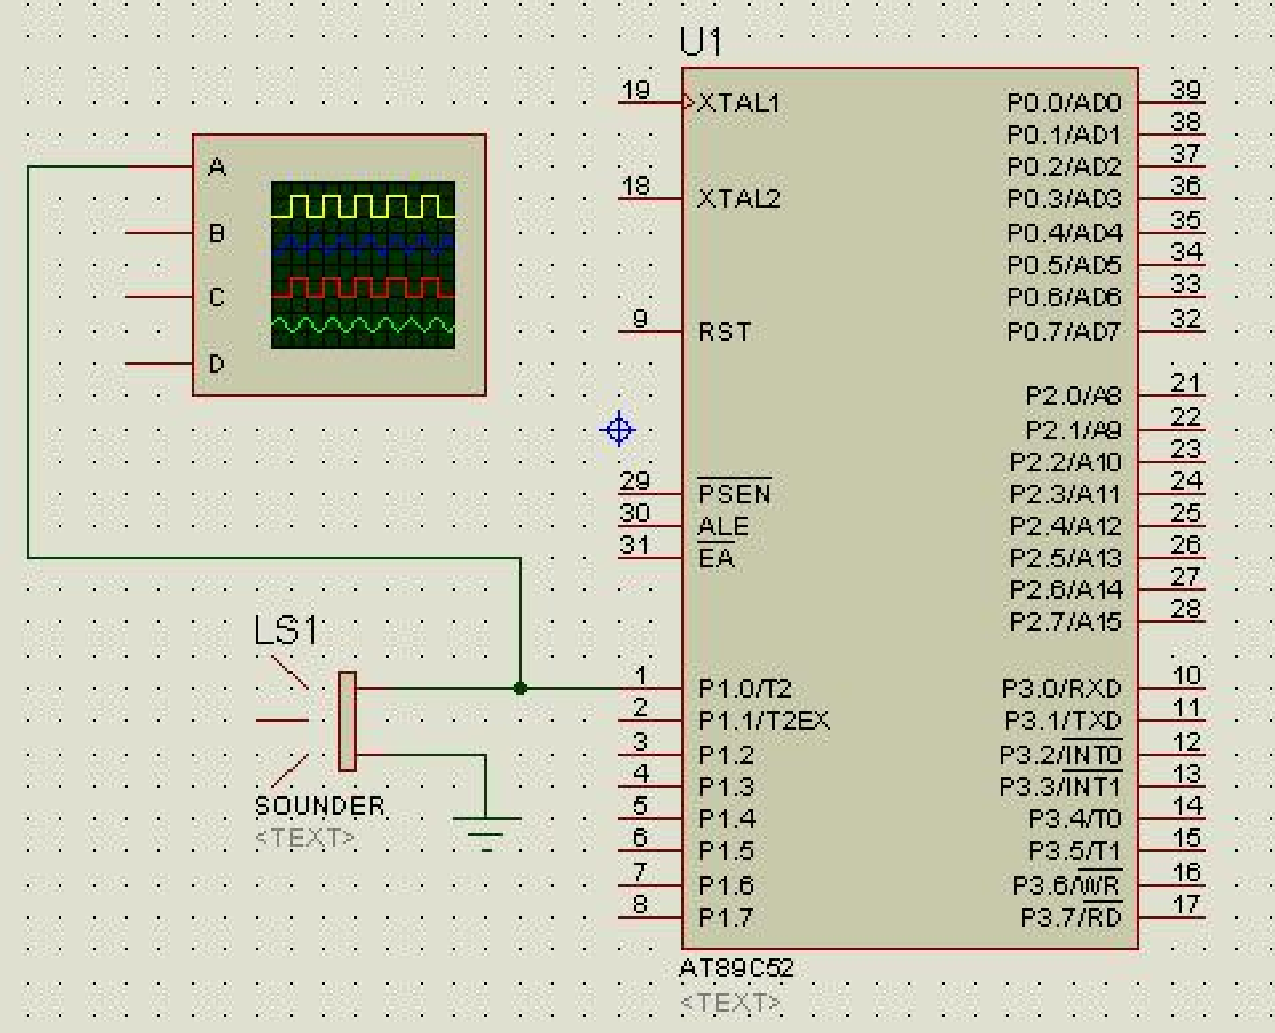
\includegraphics[width=.6\textwidth]{fig-002}
\end{center}

\subsubsection{器件清单}

\begin{tasks}(2)
  \task 单片机 STC89C52
  \task 扬声器 SOUNDER
\end{tasks}

说明:可以通过示波器观察 P1.0 口输出的方波信号,随着音高的增加,信号频
率不断增加。

\subsubsection{【参考程序】}

\begin{ccode}
#include <reg52.h>
#define uchar unsigned char

// 频率-半周期数据表 高八位
uchar code freq_h[4][7]={
   {0xF2, 0xF3, 0xF5, 0xF5, 0xF6, 0xF7, 0xF8},  //低音 1234567
   {0xF9, 0xF9, 0xFA, 0xFA, 0xFB, 0xFB, 0xFC},  //中音 1234567
   {0xFC, 0xFC, 0xFD, 0xFD, 0xFD, 0xFD, 0xFE},  //高音 1234567
   {0xFE, 0xFE, 0xFE, 0xFE, 0xFE, 0xFE, 0xFF}}; //超高音 1234567

// 频率-半周期数据表 低八位
uchar code freq_l[4][7]={
   {0x42, 0xC1, 0x17, 0xB6, 0xD0, 0xD1, 0xB6},  //低音 1234567
   {0x21, 0xE1, 0x8C, 0xD8, 0x68, 0xE9, 0x5B},  //中音 1234567
   {0x8F, 0xEE, 0x44, 0x6B, 0xB4, 0xF4, 0x2D},  //高音 1234567
   {0x47, 0x77, 0xA2, 0xB6, 0xDA, 0xFA, 0x16}}; //超高音 1234567
sbit SPK = P1^0;
void delay() //延时时间大概 100ms
{
   uchar i, j, k;
   for(i=0; i<2; i++)
   {
      for(j=0; j<170; j++)
      {
         for(k=0; k<100; k++)
         {
            ;
         }
      }
   }
}

uchar row, col;

void T0_INT() interrupt 1
{
   TH0 = freq_h[row][col];
   TL0 = freq_l[row][col];
   SPK = ~SPK;
}

void main()
{
   uchar len = 10, i;
   TMOD = 0x01;
   ET0 = 1;
   EA = 1;
   TR0 = 1;
   while(1)
   {
      for(row=0; row<4; row++)
      {
         for(col=0; col<7; col++)
         {
            TH0 = freq_h[row][col];
            TL0 = freq_l[row][col];

            for(i=len; i>0; i--)
            {
                delay();
            }
         }
      }
   }
}
\end{ccode}


\subsection{一首完整歌曲的播放}

\subsubsection{【参考程序】}

\begin{ccode}
#include <reg52.h>
#define uchar unsigned char

// 频率-定时器计数初值高 8 位
uchar code freq_h[4][7]={
   {0xF2, 0xF3, 0xF5, 0xF5, 0xF6, 0xF7, 0xF8},  //低音 1234567
   {0xF9, 0xF9, 0xFA, 0xFA, 0xFB, 0xFB, 0xFC},  //中音 1234567
   {0xFC, 0xFC, 0xFD, 0xFD, 0xFD, 0xFD, 0xFE},  //高音 1234567
   {0xFE, 0xFE, 0xFE, 0xFE, 0xFE, 0xFE, 0xFF}}; //超高音 1 2 3 4 5 6 7

// 频率-定时器计数初值低 8 位
uchar code freq_l[4][7]={
   {0x42, 0xC1, 0x17, 0xB6, 0xD0, 0xD1, 0xB6},  //低音 1234567
   {0x21, 0xE1, 0x8C, 0xD8, 0x68, 0xE9, 0x5B},  //中音 1234567
   {0x8F, 0xEE, 0x44, 0x6B, 0xB4, 0xF4, 0x2D},  //高音 1234567
   {0x47, 0x77, 0xA2, 0xB6, 0xDA, 0xFA, 0x16}}; //超高音 1 2 3 4 5 6 7

//歌曲 --《世上只有妈妈好》
uchar code song[]={
  //6,2,3 代表 6,中音,3 个半拍;
  //5,2,1 代表 5,中音,1 个半拍;
  //3,2,2 代表 3,中音,2 个半拍;
  //5,2,2 代表 5,中音,2 个半拍;
  //1,3,2 代表 1,高音,2 个半拍;
  6,2,3, 5,2,1, 3,2,2, 5,2,2, 1,3,2, 6,2,1, 5,2,1, 6,2,4,
  3,2,2, 5,2,1, 6,2,1, 5,2,2, 3,2,2, 1,2,1, 6,1,1, 5,2,1, 3,2,1, 2,2,4,
  2,2,3, 3,2,1, 5,2,2, 5,2,1, 6,2,1, 3,2,2, 2,2,2, 1,2,4,
  5,2,3, 3,2,1, 2,2,1, 1,2,1, 6,1,1, 1,2,1, 5,1,6, 0,0,0};

sbit SPK = P1^0;
uchar num = 0;
uchar row, col;

void delay()    //延时时间大概 100ms
{
  uchar i, j, k;
  for(i=0; i<3; i++)
  {
     for(j=0; j<200; j++)
     {
        for(k=0; k<200; k++)
        {
           ;
        }
     }
  }
}

void T0_INT() interrupt 1
{
  TH0 = freq_h[row][col];
  TL0 = freq_l[row][col];
  SPK = ~SPK;
}

void playMusic()
{
  uchar len, i;
  while(song[num] != 0x00)
  {
     col = song[num] - 1;
     row = song[num+1] - 1;
     len = song[num+2];
     num += 3;
     TH0 = freq_h[row][col];
     TL0 = freq_l[row][col];
     for(i=len; i>0; i--)
     {
        delay();
     }
  }
  if(song[num] == 0x00)
  {
     num = 0;
  }
  SPK = 1;
}

void main()
{
  uchar len = 4;
  TMOD = 0x01;
  ET0 = 1;
  EA = 1;
  TR0 = 1;
  while(1)
  {
     playMusic();
  }
}
\end{ccode}

【要求】对以上代码添加注释信息,描述全局变量的含义,各函数的功能,以及重要语句的
功能。

\subsection{用一个按键切换音乐的播放/停止}

在 P3.2 引脚增加一个按键,第一次按下停止播放,再次按下继续播放。仿真图
如下:

\begin{center}
  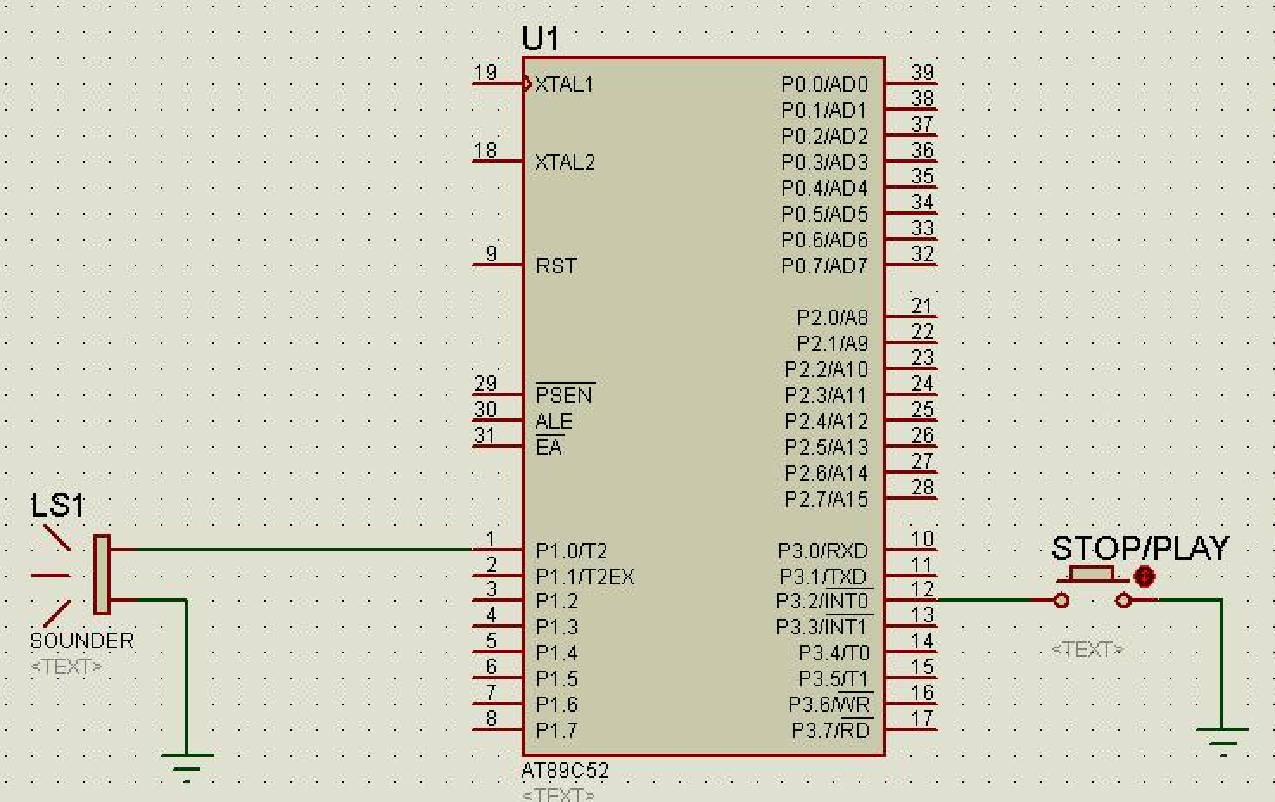
\includegraphics[width=.7\textwidth]{fig-003}
\end{center}

要求:对按键的检测使用“外部中断法”完成。

【请将编写好的 C51 程序粘贴在此处】

\begin{ccode}
int main(){
  printf("Hello, world!\n");
  return 0;
}
\end{ccode}

\subsection{播放多首歌曲}

在 P2 口接一个共阴极七段数码管,P1.3 和 P3.5 引脚增加两个按键,按
下 P1.3 引脚的键就切换到上一首歌,按下 P3.5 引脚的键就切换的到下一首歌,
同时在数码管上显示歌曲序号。电路图如下:

\begin{center}
  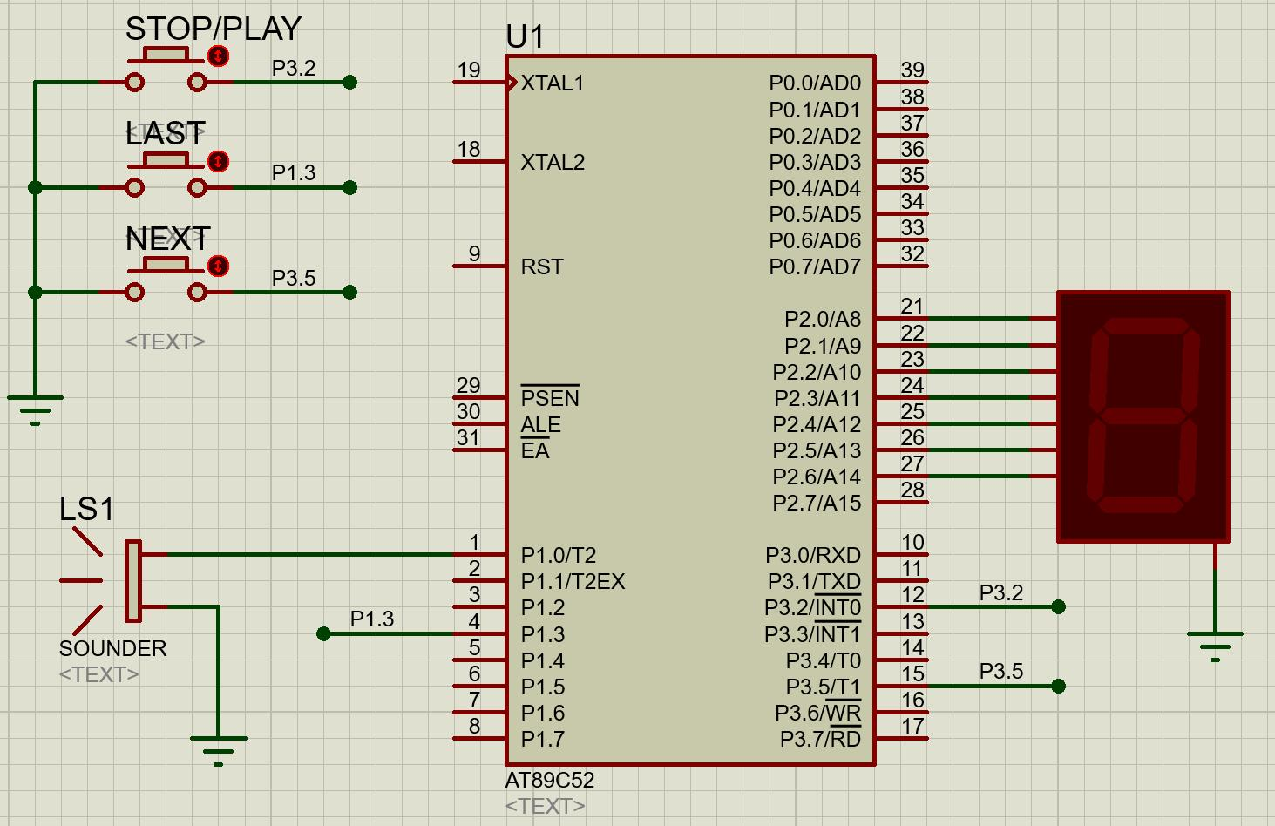
\includegraphics[width=.7\textwidth]{fig-004}
\end{center}


\subsubsection{【请将调试正确的 C51 程序粘贴在此处】}

\begin{ccode}
int main(){
  printf("Hello, world!\n");
  return 0;
}
\end{ccode}

\subsubsection{【绘制流程图】}

\begin{center}
  
\includegraphics[width=.3\textwidth]{swfulogo-emblem}
\end{center}


\subsubsection{【描述代码编写过程中遇到的问题及解决方法】}

\begin{enumerate}
\item 问题一问题一问题一

  解决方法:\zhlipsum[1]

\item 问题二问题二问题二

  解决方法:\zhlipsum[2]

\item 问题三问题三问题三
  
  解决方法:\zhlipsum[3]

\end{enumerate}

\section{PCB绘制及电路焊接}

\subsubsection{参考电路图}

\begin{center}
  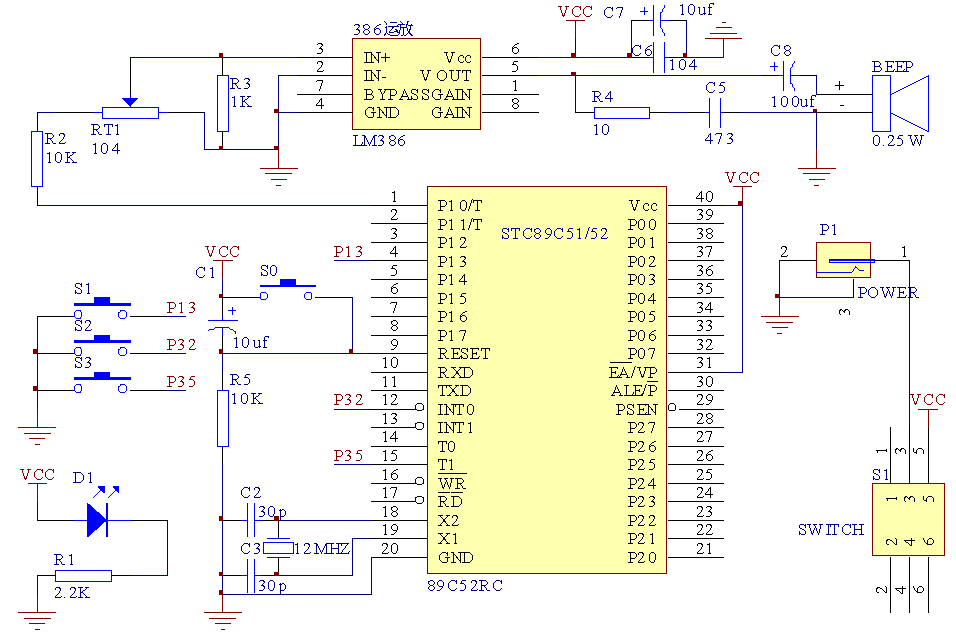
\includegraphics[width=.8\textwidth]{8-crop}
\end{center}

\subsubsection{参考 PCB 图}

\begin{center}
  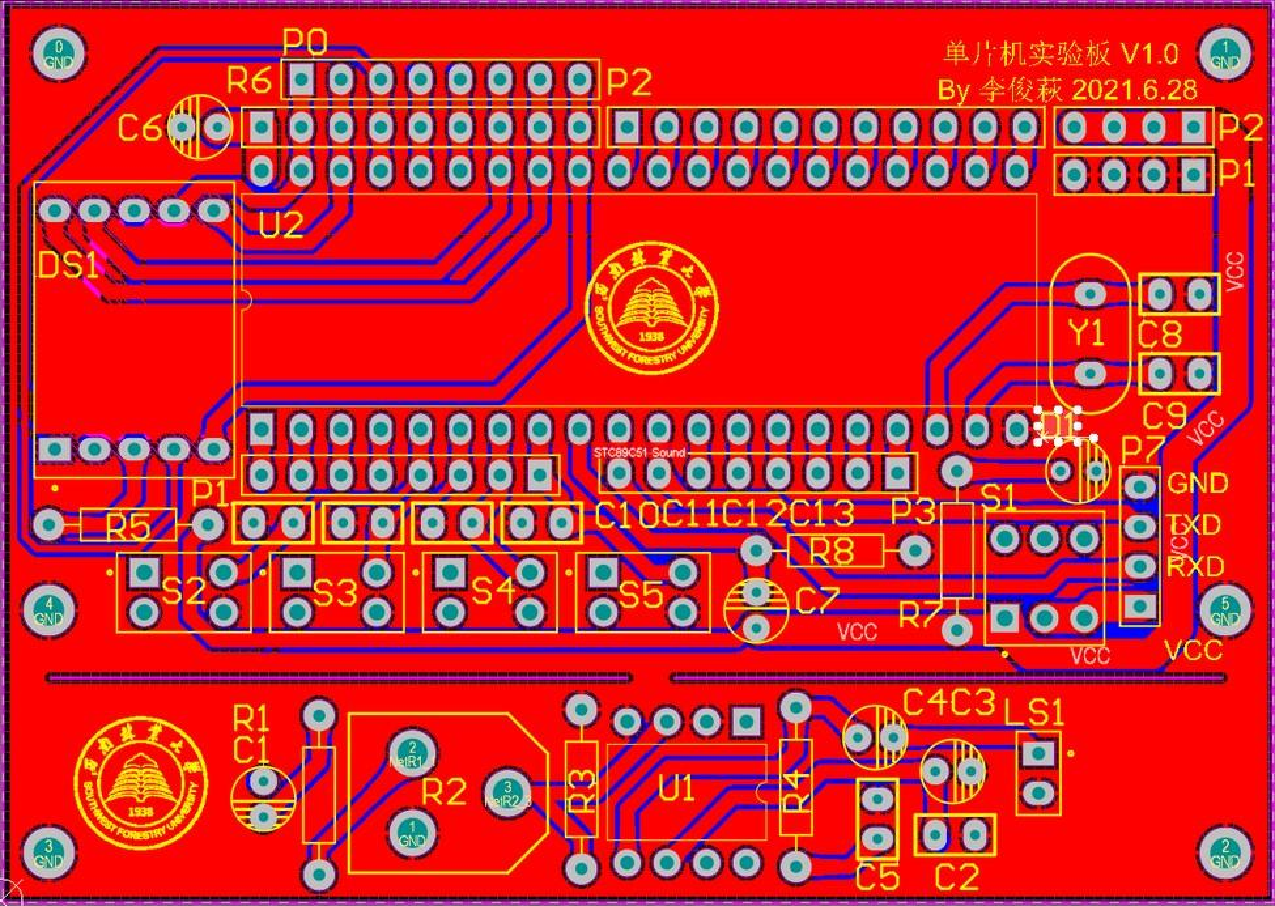
\includegraphics[width=.45\textwidth]{fig-005}\quad
  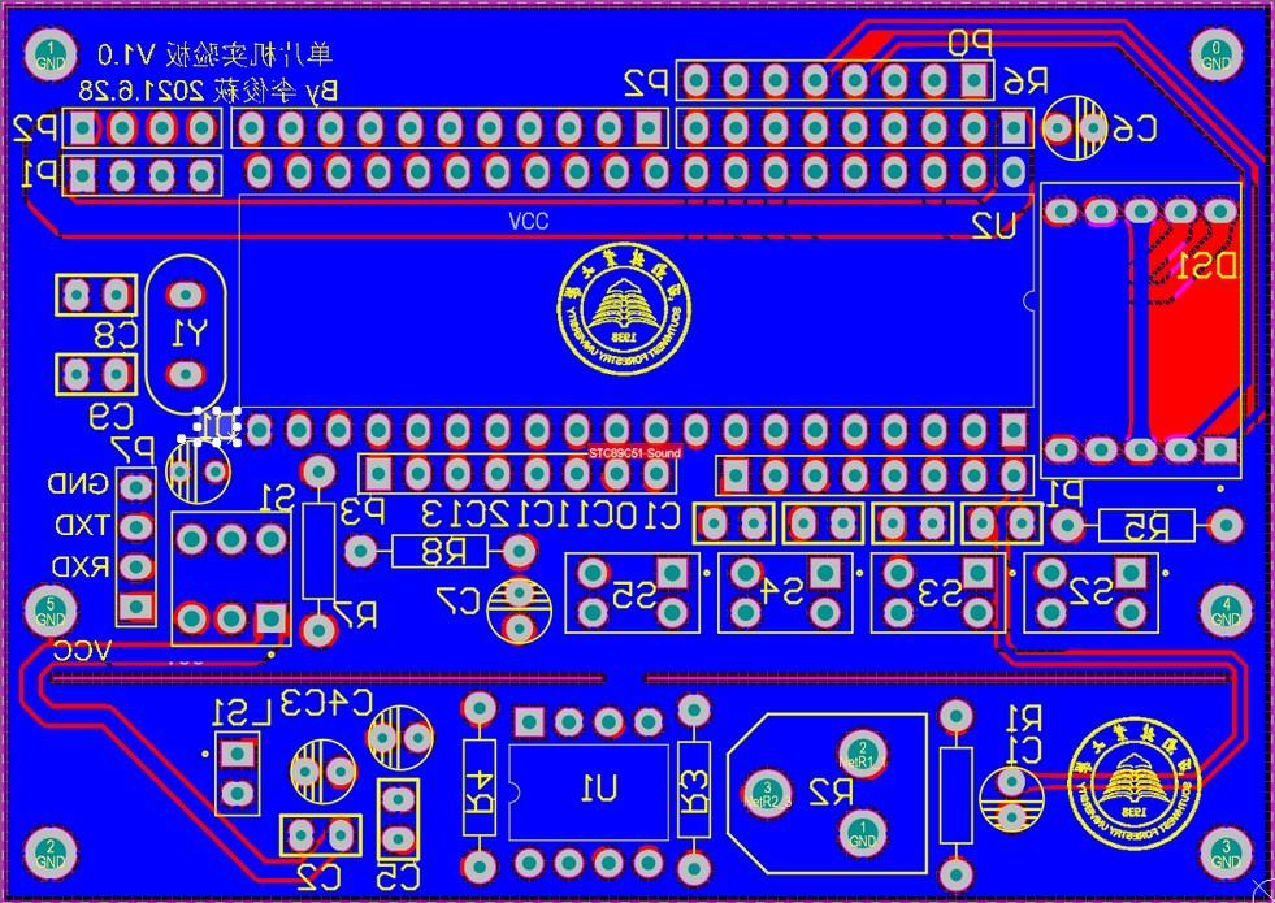
\includegraphics[width=.45\textwidth]{fig-006}
\end{center}

\subsubsection{【要求】}

\paragraph{请将自己绘制的电路原理图截图粘贴在此处}

\begin{center}
  
\includegraphics[width=.3\textwidth]{swfulogo-emblem}
\end{center}

\paragraph{请将自己绘制的 PCB 正、反面截图粘贴在此处}

\begin{center}
  
\includegraphics[width=.3\textwidth]{swfulogo-emblem}\qquad
  
\includegraphics[width=.3\textwidth]{swfulogo-emblem}
\end{center}

\paragraph{请对 PCB 板绘制过程进行简要描述}

要求:包括但不限于 PCB 板的设计流程、电气规则的设置、绘制过程中遇到的问
题及解决方法。

\zhlipsum[1-2]

\paragraph{描述实物焊接过程中遇到的问题}

\zhlipsum[3-4]

\paragraph{如何检测晶振是否起振?请描述检测过程,并将示波器检测结
  果拍照粘贴在此处}

\zhlipsum[5-6]

\paragraph{描述单片机程序烧录的过程,请将识别串口、程序下载的过程截图粘贴在此处,并简要
描述每个步骤}

\zhlipsum[7-8]

\paragraph{本次实习有什么收获和体会?请简要叙述}

\zhlipsum[9-10]



\section{照片}

\begin{enumerate}
\item 请将最终实物拍照粘贴在此处(正反面照片,背面用黑色笔写上自己的学
  号)

  \begin{center}
    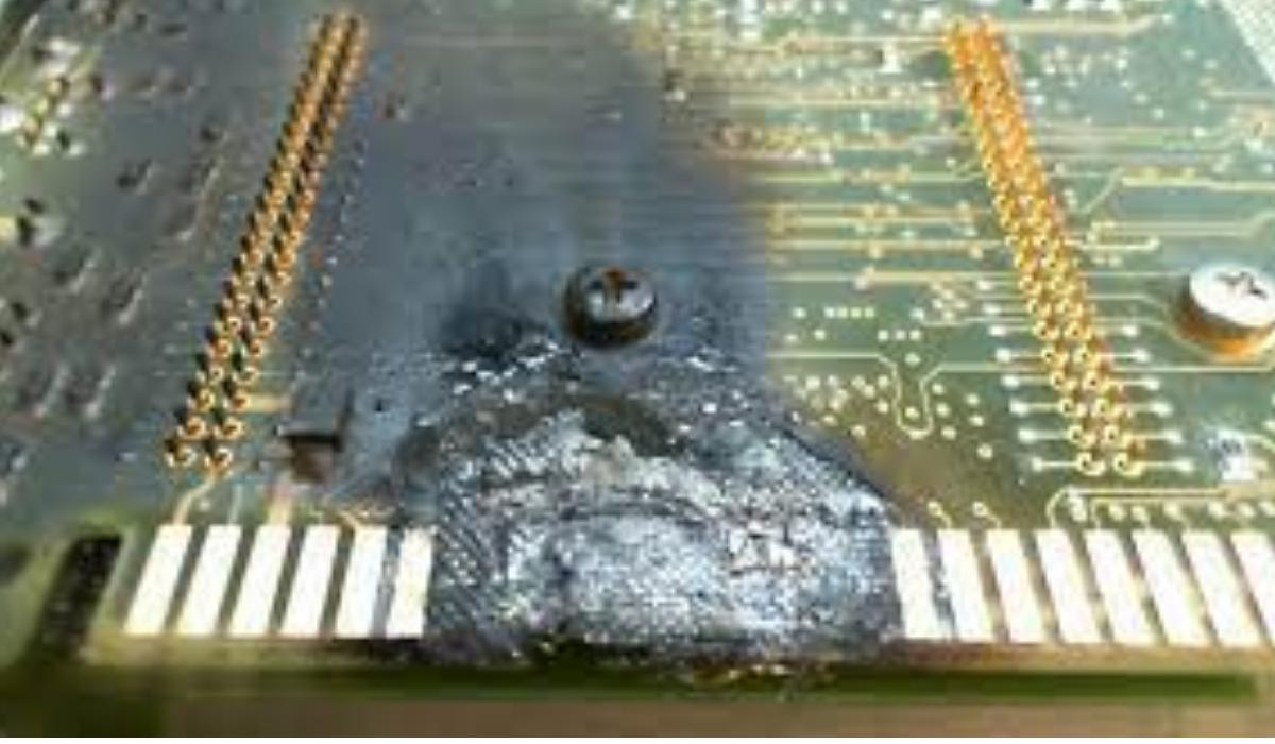
\includegraphics[width=.4\textwidth]{burnt}\qquad
    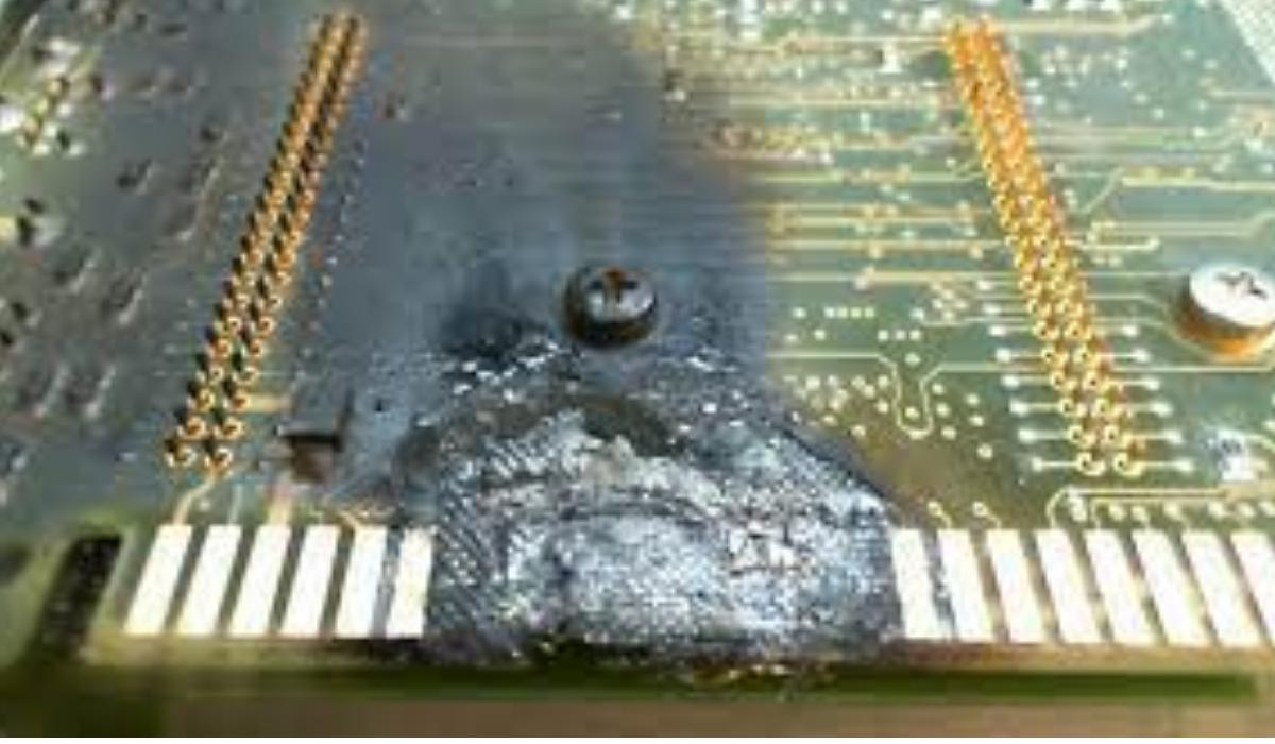
\includegraphics[width=.4\textwidth]{burnt}
  \end{center}

\item 请拍一张你焊接电路时的照片粘贴在此处。

  \begin{center}
    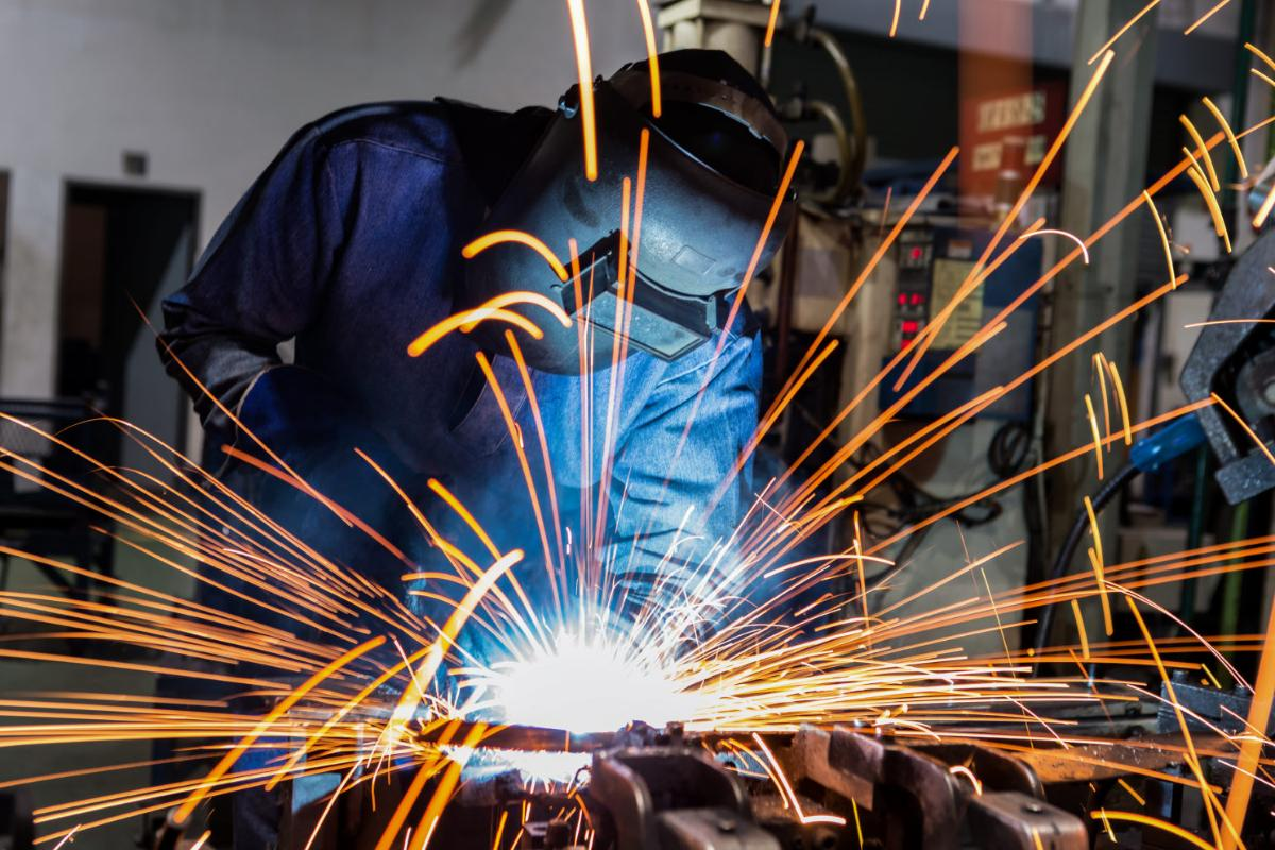
\includegraphics[width=.5\textwidth]{soldering}
  \end{center}

\end{enumerate}

\section{实习总结}

\zhlipsum[7-9]

\section{指导教师评语}

\zhlipsum[10]

\begin{flushright}
  成绩:100\\
  指导教师(签名):\\
  2024年12月21日
\end{flushright}
\end{document}
%%% Local Variables:
%%% mode: latex
%%% TeX-master: t
%%% End:
